\documentclass{article}
% !TeX spellcheck = en_US 
\usepackage[margin=2cm]{geometry}
\usepackage{makecell}
\usepackage{graphicx}
\usepackage{float}
\usepackage{caption}
\usepackage[shortlabels]{enumitem}
\usepackage{verbatim}
% \usepackage{enumerate}
\usepackage[english]{babel}

\begin{comment}
TODOs
All:
 - Think about how the printouts can be digitalized without having e.g. the police access the system.
 - Name design considerations for the DM
 - Update user wishes, stories and the like to fit the new requirements
 - Power tree and Domain Model need updating according to the new requirements
Robbin:
 - Update SSD
 - One UC should specify one session. YOu might add more than 1 item per session
 - Check reply from customer
 - A2 Special Overflows.
Oli:
 - Update SSD
 x Specify in UC title what you are updating
 ? One UC should specify one session. YOu might update more than 1 item per session
 x Stakeholders and interests box overflows on the left. Use \makecell[l]{text1//text2} for multiline text in tabular
 x ``Frequency of occurence: Frequent'' <-- seriously?!
 x Specify what transaction you are starting and with what parameters
 x ``information'' is ambiguous and non-specific. Use parameters instead.
 x Updated bb-SD B1
 - Usecase B2
 - bb-SD B2
 - gb and wb for C1
 - gb and wb for A2
  
Nicu:
 - Update SSD
 - Specify in UC title what you are deleting
 - One UC should specify one session. YOu might delete more than 1 item per session
 - Honestly, just check the pictures. Theres some many comments and remarks.
\end{comment}

\DeclareUnicodeCharacter{20AC}{-}
\begin{document}

\setcounter{secnumdepth}{0}

\hbox{
	\hspace*{0.08\textwidth}
	\rule{0.5pt}{\textheight}
	\hspace*{0.001\textwidth}
	\rule{0.5pt}{\textheight}
	\hspace*{0.05\textwidth}
	\parbox[b]{0.75\textwidth}{
		{\noindent\huge\bfseries Problem Analysis \& Software Design \\}\\[2\baselineskip] % Title
		\large{
		\textbf{Group:} 9\\[\baselineskip]
		\begin{tabular}{@{}l l l l@{}}
			\textbf{Names:}& (A) Robbin de Groot  &\textbf{S-number:} &s3376508\\
			& (B) Oliver Strik  & &s3100693\\
			& (C) Nicu Ghidirimschi & & s3197395
		\end{tabular}}\\

		\vspace{6pt}
		{\large \textbf{Report:} Iteration 2 } \\[\baselineskip] % Tagline or further description
		{\large \textbf{Date:} \today } \\[4\baselineskip] % Tagline or further description
		{\large \textsc{ Prof. E.O. de Brock \& Dr. R. Smedinga }}
	\vspace{0.40\textheight} % Whitespace between the title block and the publisher
	{\Large\noindent \\ Computing Science - Year 2 \vspace{0.7cm}
	\Large\noindent \\University of Groningen \vspace{5pt}\\ \large Faculty of Science \& Engineering }}
}
\newpage

%%% index page
\tableofcontents

\section{Introduction}
An auctioning company called ``The AuctionHouse\textsuperscript{TM}'' auctions provided goods to customers. Currently, they auction and display the goods in a warehouse just outside of city limits. Owner John wants to automate the administration of auctions and other activities using an IT solution as well as introduce some new services made possible by such a system.

\section{Expectations Summary and Conclusion}
John wants the sellers to be able to register their goods in the to-develop-system. These goods then need to be assessed and possibly removed if they lack the requirements. A couple of days before an auction, potential customers must be able to view the goods. The goods are then auctioned at location (so not through the system).\\
Currently, regular customers get mail informing them of the goods on sale, rather than having to go and see the available goods in person.\\
Payments are done through cash or card, and not through credit cards. Bigger customers get offered a special billing procedure.
The police is handed a list of goods on auctions, so they can identify any stolen goods.
Once the system is completed, a system administrator should make sure every person has the right permissions for the system, and verify that it is operating properly.

\section{Potential users and user wishes}
\subsection{Actors and Users}
What follows is a list of user (groups) that need to interact with the system directly. Also is a brief description of the wishes in customer language. This analysis is made before the analysis of the problem and design of the system, and therefore will not include any new roles that surface later on.\\
This list can also function as a dictionary for the upcoming analysis.
\begin{itemize}[noitemsep]
	\item Owner of The AuctionHouse\textsuperscript{TM} (John)\\
		The owner needs to be able to manage the staff members and their access and permissions in the system. The owner also wants to file the search requests he gets from the customers.
		The owner needs to be able to manage the staff members and their access and permissions in the system. The owner also wants to file the search requests he gets from the customers.
	\item Secretary\\
		The secretary handles some basic customer services that do not require a special role within the company. The secretary wants to register customers and sellers in the system so their credentials are saved. Currently, the secretary is also responsible for printing out the various lists that need to be distributed, like the list of items for the police. The secretary may also want to modify simple attributes of the items already in the system in case, for example, a seller wants to increase the minimum price they want for their product.
	\item Purchasing agent\\
		The purchasing agent wants to evaluate the presented goods for possible sale, and if they will be auctioned, needs to make sure they are being stored in the storehouse (which does not necessarily have to be done through the system).
	\item Private Individuals and Merchants (Owners/Sellers of the goods)\\
		Sellers need to be able to present their goods to the purchasing agent so he/she can decide whether they can be auctioned.
	\item Customers/Buyers\\
		Customers want to see the list of goods on sale, see the date they are auctioned at and potentially buy them. They also want to be able to make a request for the search of a specific item.
	\item Viewers/The public\\
		Viewers want to see the products that are going to be auctioned, and therefore need to have access to the list of goods along with their price and auctioning date(s).
	\item System Administrator\\
		The system administrator is responsible for the system's behaviour and needs to monitor system activity.
\end{itemize}

\subsection{Other Stakeholders}
Below is the list of stakeholders; people who have interests in the development of the system, or are otherwise involved with it, while not having to interface with it directly or having additional needs compared to other user groups.
\begin{itemize}[noitemsep]
	\item Regular Customer\\
		Regular customers have no extra needs or wishes. However, they are registerd in the system with their credentials and receive auction catalogues at their home address and, if they like, a list of available goods in their catagory of interest.
	\item Big Customer\\
		Big customers are essentially normal customers, but since their expenses are greater, they are offered a special billing procedure.
	\item Police\\
		The police has no need to directly access the system. However, they are offered a list (printout) of goods to follow potentially stolen goods. This list may be digitalized later in development.
\end{itemize}

\subsection{User Wishes and Stories}
Users and stakeholders need the system to be able to handle their requests. Below is a list of those wishes.
\begin{itemize}[noitemsep]
	\item Administrators: do everything below under test environments
	\item Owner: add/remove/modify/view staff members
	\item Owner: *\underline{create search request}
	\item Purchasing Agent: \underline{register}/\underline{modify} items for sale
	\item Auctioneer: mark item as sold/junk
	\item Auctioneer: \underline{delete item from the item list}
	\item Secretary: registers customers and sellers to the system
	\item Secretary: generate printouts of items for sale/sold/etc.
	\item Secretary: modify basic parameters of items (e.g. modify the auction date of an item).
	\item Secretary: \underline{register customers in the system as ``regular customers''.}
	\item Seller: view items they have for sale
	\item Seller: view items they have sold
	\item Buyer: view items they have bought
	\item Buyer: request the search for an item
	\item Public: view items that are for sale
	\item Public: view auction schedule
	\item Public: \underline{reserve books}
\end{itemize}
Legend: \underline{underlined}: User wish is made into a use case. `*': a new requirement that is introduced because of the system-to-be's existence.\\\\
To visualize this, a diagram is provided. This diagram is a ``power tree'' that shows how permissions are divided and who can do the same as another user group.
\begin{figure}[H]
	\centering
	% ignore the compilation warning, it has to do with the pdf and the graphicx package not accounting for some variable within the file, even though the variable has had no purpose for about 10 years now. #research
	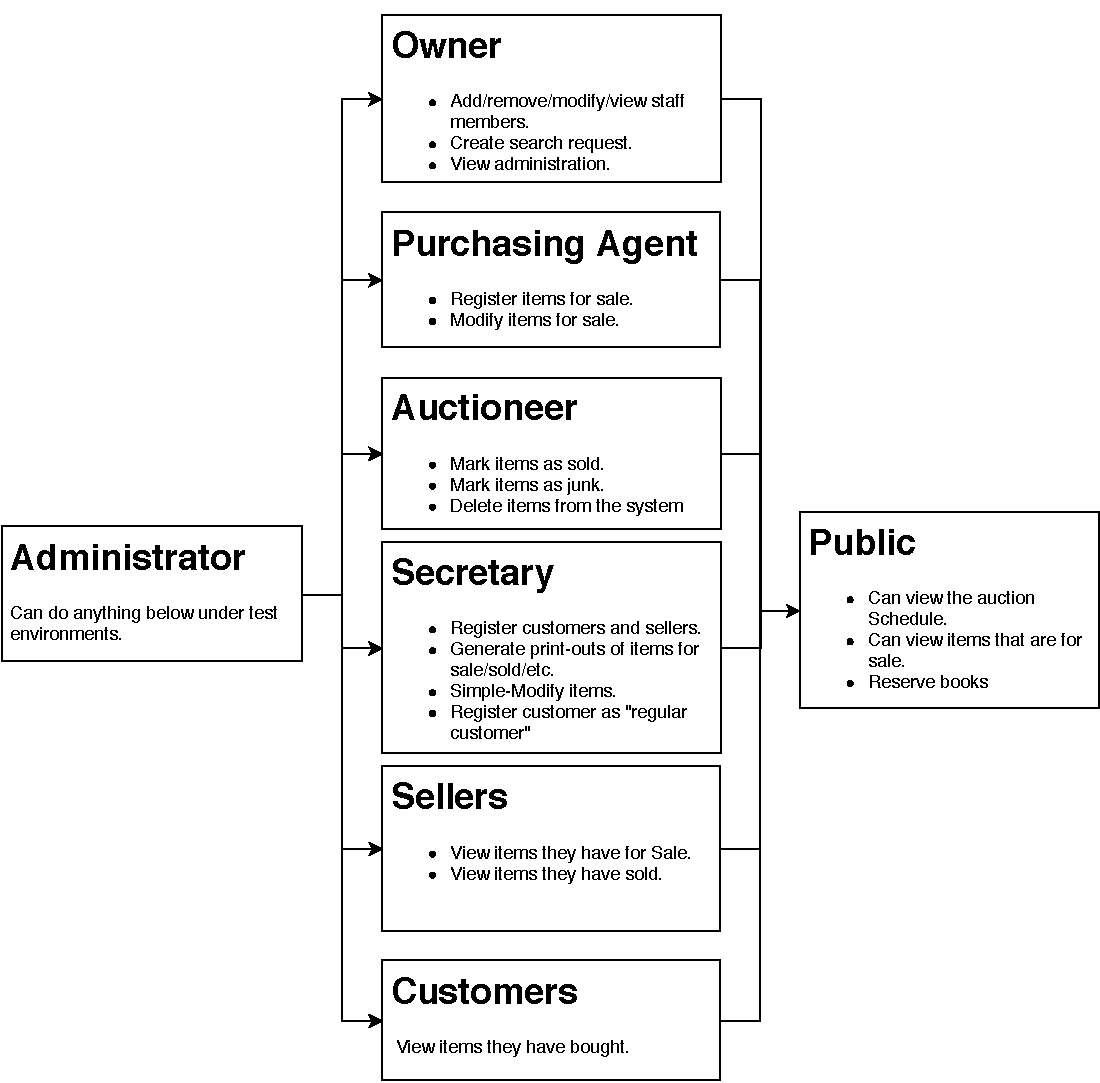
\includegraphics[scale=.75]{uml/power_tree.pdf}
	\caption*{A power tree showing the relations between user groups and permissions. Arrows indicate what permissions are inherited. For example, the Owner, Purchasing Agent, Auctioneer, etc. can all do what the public can, with some class specific permissions.}
\end{figure}




\section{Use Cases}
% layout and sectioning from Slides week 1, page 25
\subsection{Create and add an item - (A1)}
\subsubsection*{Analysis}
\begin{tabular}{@{}l l}
\textbf{Scope}:&The AuctionHouse\textsuperscript{TM} automated administration system\\
\textbf{Level}:&User goal\\
\textbf{Primary Actor}:&Purchasing Agent\\
\textbf{Stakeholders and Interests}:&\begin{tabular}[t]{@{}l}Purchasing Agent: wants to enter parameters easily and quickly\\Seller: wants his goods to be visible to potential buyers\end{tabular}\\
\textbf{Preconditions}:&Purchasing agent is identified and authenticated.\\
\textbf{Postconditions}:&\begin{tabular}[t]{@{}l}The item has been added to the system, or a failure was returned.\\The product has been registered for an upcoming auction.\\The item is (or will become) visible for potential buyers\\and the otherwise authorized.\end{tabular}\\
\textbf{Special requirements}:&A list of categories and a list of future auction dates needs to available in the system\\
\textbf{Frequency of occurence}:& \begin{tabular}[t]{@{}l}Depedent on the amount of sellers and auctions per month.\\Since there is 1 auction per month. If we expect about 30 sellers, then there\\are 30 occurences per month, so about 1 per day.\end{tabular}
\end{tabular}\\\\
\textsl{Main Success Scenario}
\begin{enumerate}[noitemsep]
	\item The user starts the `add item' transaction with the system, having all parameters of the item to be added ready.
	\item The system provides the user with a list of categories to choose from, and a list of future planned aution dates.
	\item The user provides all necessary parameters and chooses a category for the item, and an auction date. The parameters to provide are:
	\begin{itemize}[noitemsep]
		\item The amount of the item available
		\item The type of item
		\item A description
		\item If the item possesses any antiquarian value
		\item A minimum price decided by the owner
		\item The date when brought in
		\item Name and address of the owner plus identification
		\item Planned auction date
		\item Distinguishing features
	\end{itemize}
	\item The system adds the item with all provided parameters to the list and generates an Item ID unique to the item.
	\item The system returns to the user with a confirmation message containing the generated item ID, or a failure.
\end{enumerate}
\textsl{Extensions}
\begin{itemize}[noitemsep]
	\item When a failure is returned, the system state remains unchanged; no item or other parameters was added.
	\item When not all required parameters were provided, the system will first ask the user to provide it until all parameters is provided.
\end{itemize}
\textsl{System Sequence Diagram}
\begin{figure}[H]
	\centering
	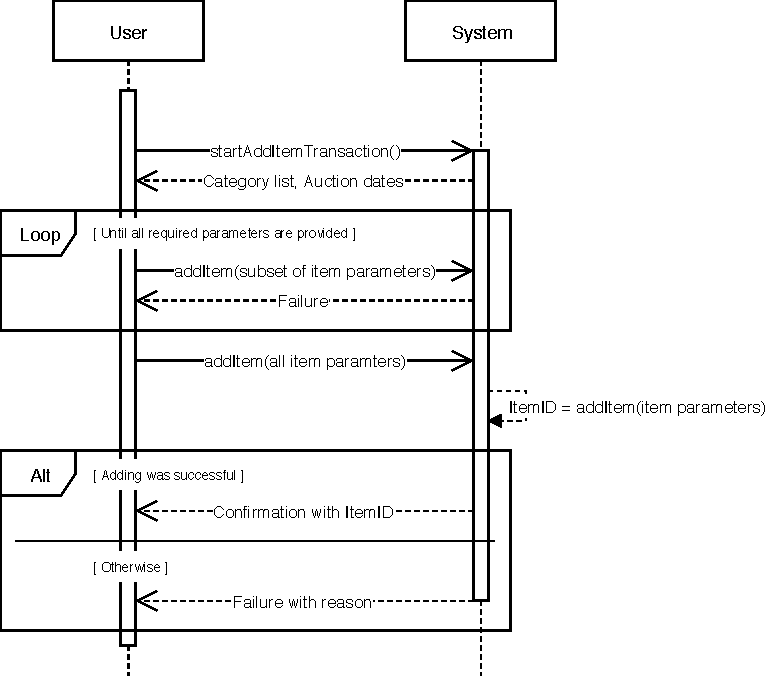
\includegraphics[scale=1]{SD-bb-create.pdf}
	\caption*{Interactions displayed in a System Sequence Diagram defined by the MSS and its extensions in blackbox format}
\end{figure}
\subsection{Create and add a user - (A1)}
\subsubsection*{Analysis}
\begin{tabular}{@{}l l}
\textbf{Scope}:&The AuctionHouse\textsuperscript{TM} automated administration system\\
\textbf{Level}:&User goal\\
\textbf{Primary Actor}:&Owner \& Secretary\\
\textbf{Stakeholders and Interests}:&\begin{tabular}[t]{@{}l}Owner: wants to register his staff to the system.\\Secretary: wants to register buyers and sellers to the system.\\Staff, Buyers and Sellers: Want to be granted access to the system.\end{tabular}\\
\textbf{Preconditions}:&User is identified and authenticated.\\
\textbf{Postconditions}:&\begin{tabular}[t]{@{}l}A new user has been registered to the system.\\The person for whom a new user has been added received\\the necessary authorization credentials for the system.\end{tabular}\\
\textbf{Special requirements}:&A list of categories and a list of future auction dates needs to available in the system\\
\textbf{Frequency of occurence}:& \begin{tabular}[t]{@{}l}Depedent on the amount of job applications and new buyers and sellers per month.\\Since not many staff members at required, the former will be rare, say 1 per month.\\The latter will be more common, say 10 times per month. That is an estimated\\11 times per month.\end{tabular}
\end{tabular}\\\\
\textsl{Main Success Scenario}
\begin{enumerate}[noitemsep]
	\item The user starts the `add user' transaction with the system, having all parameters of the user to be added ready.
	\item The system confirms the interaction and asks the user to provide all the necessary parameters.
	\item The user provides all necessary parameters. The parameters to provide are (optional parameters are marked with a `*'):
	\begin{itemize}[noitemsep]
		\item The name of the new user (username)
		\item The class of the new user (e.g. Staff member, Buyer, Seller)\\
		\quad The selection depends on the user doing the transaction
		\item The address of the person bound to the new user
		\item * An email address (for digital mail)
		\item * A bank account number for deposits/sallary
	\end{itemize}
	\item The system creates the user with all provided parameters and adds it to the list. It also generates authentication credentials for the person bound to the new user.
	\item The system returns to the user with a confirmation message containing the generated authentication credentials, or a failure.
\end{enumerate}
\textsl{Extensions}
\begin{itemize}[noitemsep]
	\item When a failure is returned, the system state remains unchanged; no user or other parameters was added.
	\item When not all required parameters were provided, the system will first ask the user to provide it until all parameters is provided.
	\item The system will only provide the classes for the new user based on the class of the user who is doing the transaction.
\end{itemize}
\textsl{System Sequence Diagram}
\begin{figure}[H]
	\centering
	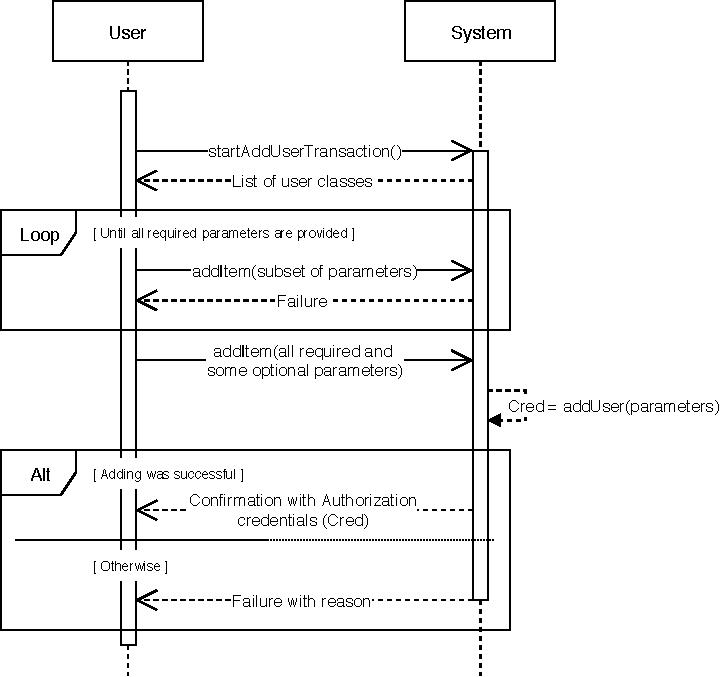
\includegraphics[scale=1]{SD-bb-createuser.pdf}
	\caption*{Interactions displayed in a System Sequence Diagram defined by the MSS and its extensions in blackbox format}
\end{figure}

\subsection{Updating an item - (B1)}
\subsubsection*{Analysis}
\begin{tabular}{@{}l l}
\textbf{Scope}:&
The AuctionHouse\textsuperscript{TM} automated administration system\\
\textbf{Level}:&
User goal\\
\textbf{Primary Actor}:&
Purchasing Agent, Auctioneer, Secretary\\
\textbf{Stakeholders and Interests}:&
\begin{tabular}[t]{@{}l}
Purchasing Agent, Auctioneer, Secretary: wants to update ??? an item's\\
parameters ??? quickly and easly
\end{tabular}\\
\textbf{Preconditions}:&
Actor is identified and authenticated.\\
\textbf{Postconditions}:&
\begin{tabular}[t]{@{}l}
The item has been updated on the system, or a failure was returned.\\
The updates to the item's parameters are (or will become) visible for potential\\
 buyers and the otherwise authorized.
\end{tabular}\\
\textbf{Special requirements}:&
\begin{tabular}[t]{@{}l}
The current parameters of an item and a list of future auction dates needs\\
to available in the system.
\end{tabular}\\
\textbf{Frequency of occurence}:&
\begin{tabular}[t]{@{}l}
Daily. Dependent on how many mistakes the purchasing agent makes when\\
entering an item, how often a seller wishes to change something about their\\
items (via the secretary) and how many auctions there are where auctioneers\\
 need to mark the item as sold or junk.
\end{tabular}\\
\end{tabular}\\\\
\textsl{Main Success Scenario}
\begin{enumerate}[noitemsep]
	\item The user starts the update item transaction, with all parameters to be updated ready.
	\item The system provides the user with the current parameters of the item that they are authorised to edit.
	\item The user provides the updated parameters. The parameters that can be updated are:
	\begin{itemize}[noitemsep]
		\item The amount of the item available
		\item The type of item
		\item A description
		\item If the item possesses any antiquarian value
		\item A minimum price decided by the owner
		\item The date when brought in
		\item Name and address of the owner plus identification
		\item Planned auction date
		\item Distinguishing features
	\end{itemize}
	\item The system updates the item with the given parameters.
	\item The system returns to the user whether it was successful.
\end{enumerate}
\textsl{Extensions}
\begin{itemize}[noitemsep]
	\item If unsucessful, the system database remains unchanged; no item or other parameters was added or changed.
\end{itemize}
\textsl{System Sequence Diagram}
\begin{figure}[H]
	\centering
	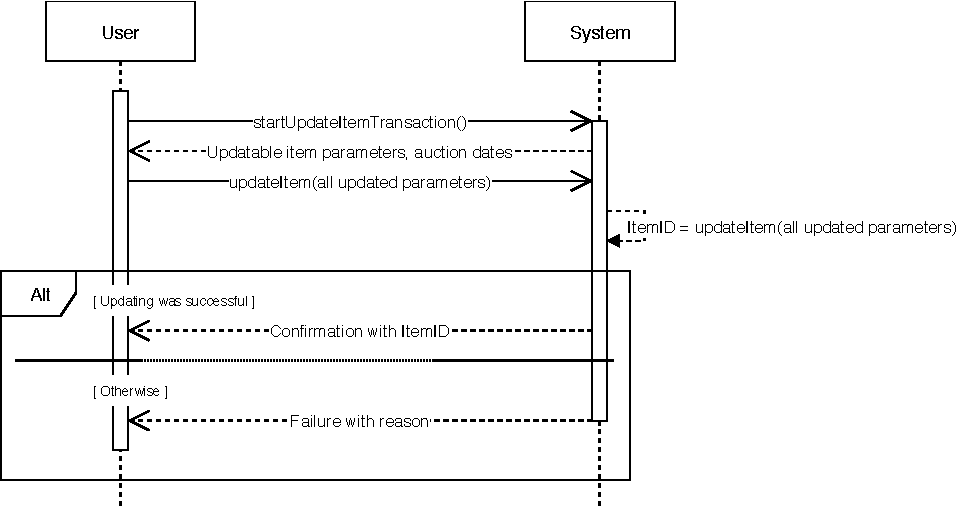
\includegraphics[scale=1]{SD-bb-update.pdf}
	\caption*{Interactions displayed in a System Sequence Diagram in blackbox format}
\end{figure}

\subsection{Deleting - (C1)}
\subsubsection*{Analysis}
\begin{tabular}{@{}l l}
\textbf{Scope}:&The AuctionHouse\textsuperscript{TM} automated administration system\\
\textbf{Level}:&User goal\\
\textbf{Primary Actor}:&Auctioneer\\
\textbf{Stakeholders and Interests}:&\begin{tabular}[t]{@{}l}Auctioneer: Wants to remove items that are not stored in the stockroom from the item list;
\\Owner: Does not want to display non-existent items to the viewers;
\\Viewer: Wants to see only existent items and (if applicable) their actual quantity.  \end{tabular}\\
\textbf{Preconditions}:&\begin{tabular}[t]{@{}l}Actor is identified and authenticated.\\Item has been already removed from the stockroom but is still present in the item list.\end{tabular}\\
\textbf{Postconditions}:&\begin{tabular}[t]{@{}l}The item list has been updated and does not contain the removed item. \end{tabular}\\
\textbf{Special requirements}:&\begin{tabular}[t]{@{}l}The item should be identifiable (perhaps with an unique identification number).\end{tabular}\\
\textbf{Frequency of occurence}:&Very frequent after each auction (once per month), otherwise rarely to even none at all.\\
\end{tabular}\\\\
\textsl{Main Success Scenario}
\begin{enumerate}[noitemsep]
	\item The user enters the deletion mode.
	\item The system displays a filterable list of all items.
	\item (Optional) The user filters the list using the following items characteristics:
	\begin{itemize}[noitemsep]
		\item The amount of the item available
		\item The type of item
		\item A description
		\item If the item possesses any antiquarian value
		\item A minimum price decided by the owner
		\item The date when brought in
		\item Name and address of the owner plus identification
		\item Planned auction date
		\item Distinguishing features
	\end{itemize}
	\item The user selects an item from the resultant list.
	\item If the item is already in the  "selected for deletion" list remove it and jump to 8.
	\item The systems prompts the user if the item is surely removed from the stockroom.
	\item If the user answers yes - add the item to the "selected for deletion" list, otherwise do nothing.
	\item If the user wants to modify the "selected for deletion" list, repeat steps 2-8.
	\item Remove all items in the "selected for deletion" list from the item list and display the number of overall deleted items.
\end{enumerate}
\textsl{Extensions}
\begin{itemize}[noitemsep]
	\item If the "selected for deletion" list is empty, no changes are made to the original item list.
	\item For homogeneous items that share the same catalog item, decrease the quantity accordingly instead of removing the whole item from the list in case not all items are removed from the stockroom.  \\
\end{itemize}
\textsl{System Sequence Diagram}\\\\
\begin{figure}[H]
	\centering
	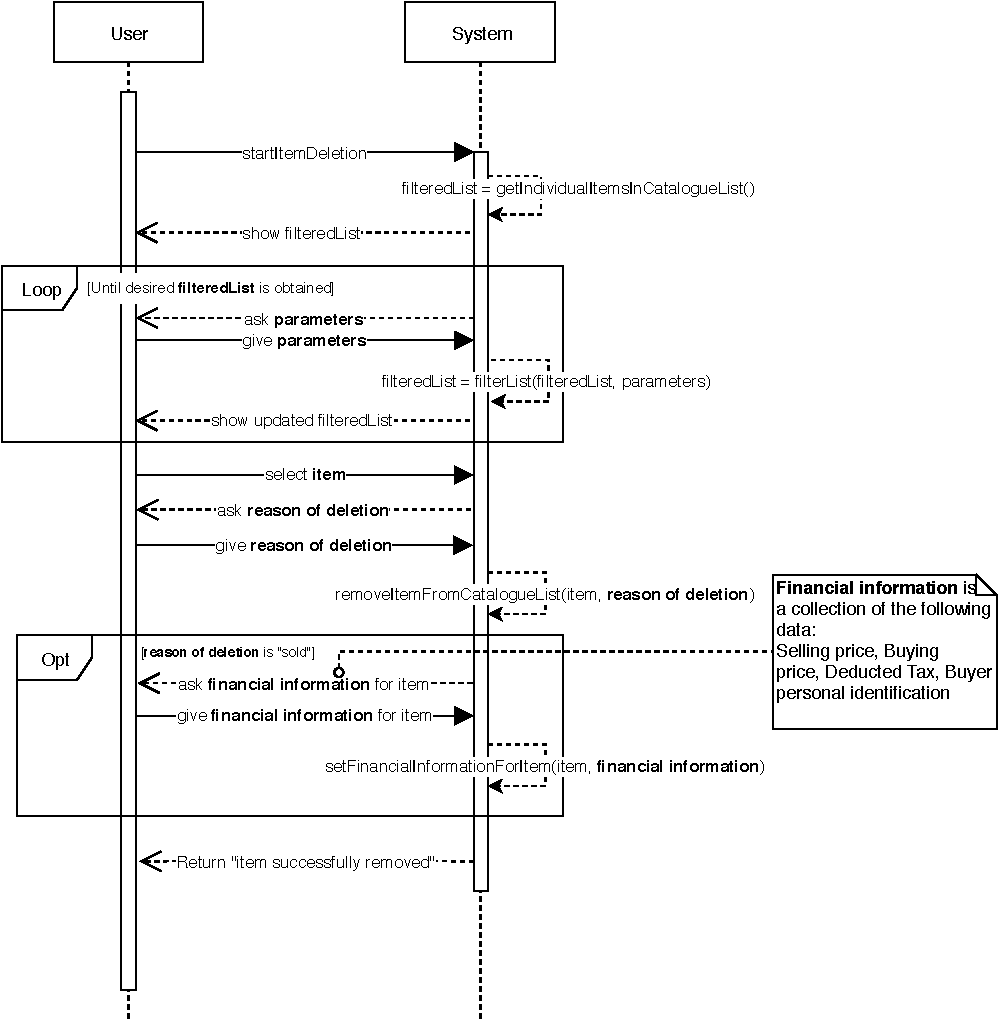
\includegraphics[scale=1]{uml/SD-bb-delete.pdf}
	\caption*{Interactions displayed in a System Sequence Diagram defined by the MSS and its extensions in blackbox format.}
\end{figure}

\subsection{Create a Search Service Request - (A2)}
\subsubsection*{Analysis}
\begin{tabular}{@{}l l}
\textbf{Scope}:&The AuctionHouse\textsuperscript{TM} automated administration system\\
\textbf{Level}:&User goal\\
\textbf{Primary Actor}:&Owner\\
\textbf{Stakeholders and Interests}:&\begin{tabular}[t]{@{}l}Owner: wants to register the search request.\\Buyers: want their search request to be registered by the owner.\end{tabular}\\
\textbf{Preconditions}:&User is identified and authenticated.\\
\textbf{Postconditions}:&\begin{tabular}[t]{@{}l}The search request is registered in the system.\\The buyer is notified of confirmation or failure.\end{tabular}\\
\textbf{Special requirements}:&A yearly fee of €20 must be paid for the service to process the request. The system should check whether this is in order.\\
\textbf{Frequency of occurence}:& \begin{tabular}[t]{@{}l}TODO\end{tabular}
\end{tabular}\\\\
\textsl{Main Success Scenario}
\begin{enumerate}[noitemsep]
	\item The user starts the `file search request' transaction for a buyer with the system, having all parameters of the user to be added ready.
	\item The system confirms the buyer has paid the yearly fee
	\item The system confirms the interaction and asks the user to provide an item catalogue and a maximum price.
	\item The user provides these parameters.
	\item The system creates the search request with the item catalogue,the maximum price and the buyer interested and adds it to the list. The system also generates a Search ID for reference.
	\item The system informs the buyer that the request has been made.
	\item The system returns to the user with a confirmation message containing the Search ID, or a failure.
\end{enumerate}
\textsl{Extensions}
\begin{itemize}[noitemsep]
	\item If the yearly fee has not been paid, the system will return a failure and ends the transaction.
	\item When a failure is returned, the system state remains unchanged; no search request or other parameters was added.
	\item When not all required parameters were provided, the system will first ask the user to provide it until all parameters is provided.
\end{itemize}
\textsl{System Sequence Diagram}
\begin{figure}[H]
	\centering
	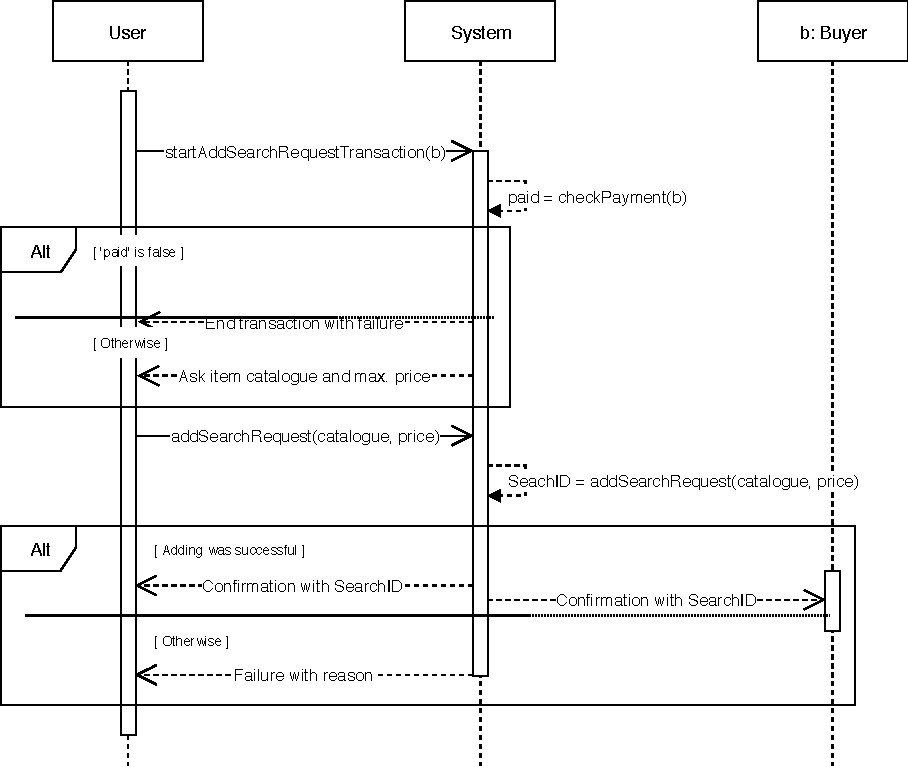
\includegraphics[scale=1]{SD-bb-createsearch.pdf}
	\caption*{Interactions displayed in a System Sequence Diagram defined by the MSS and its extensions in blackbox format}
\end{figure}


\section{Domain Model}
\begin{figure}[H]
	\centering
	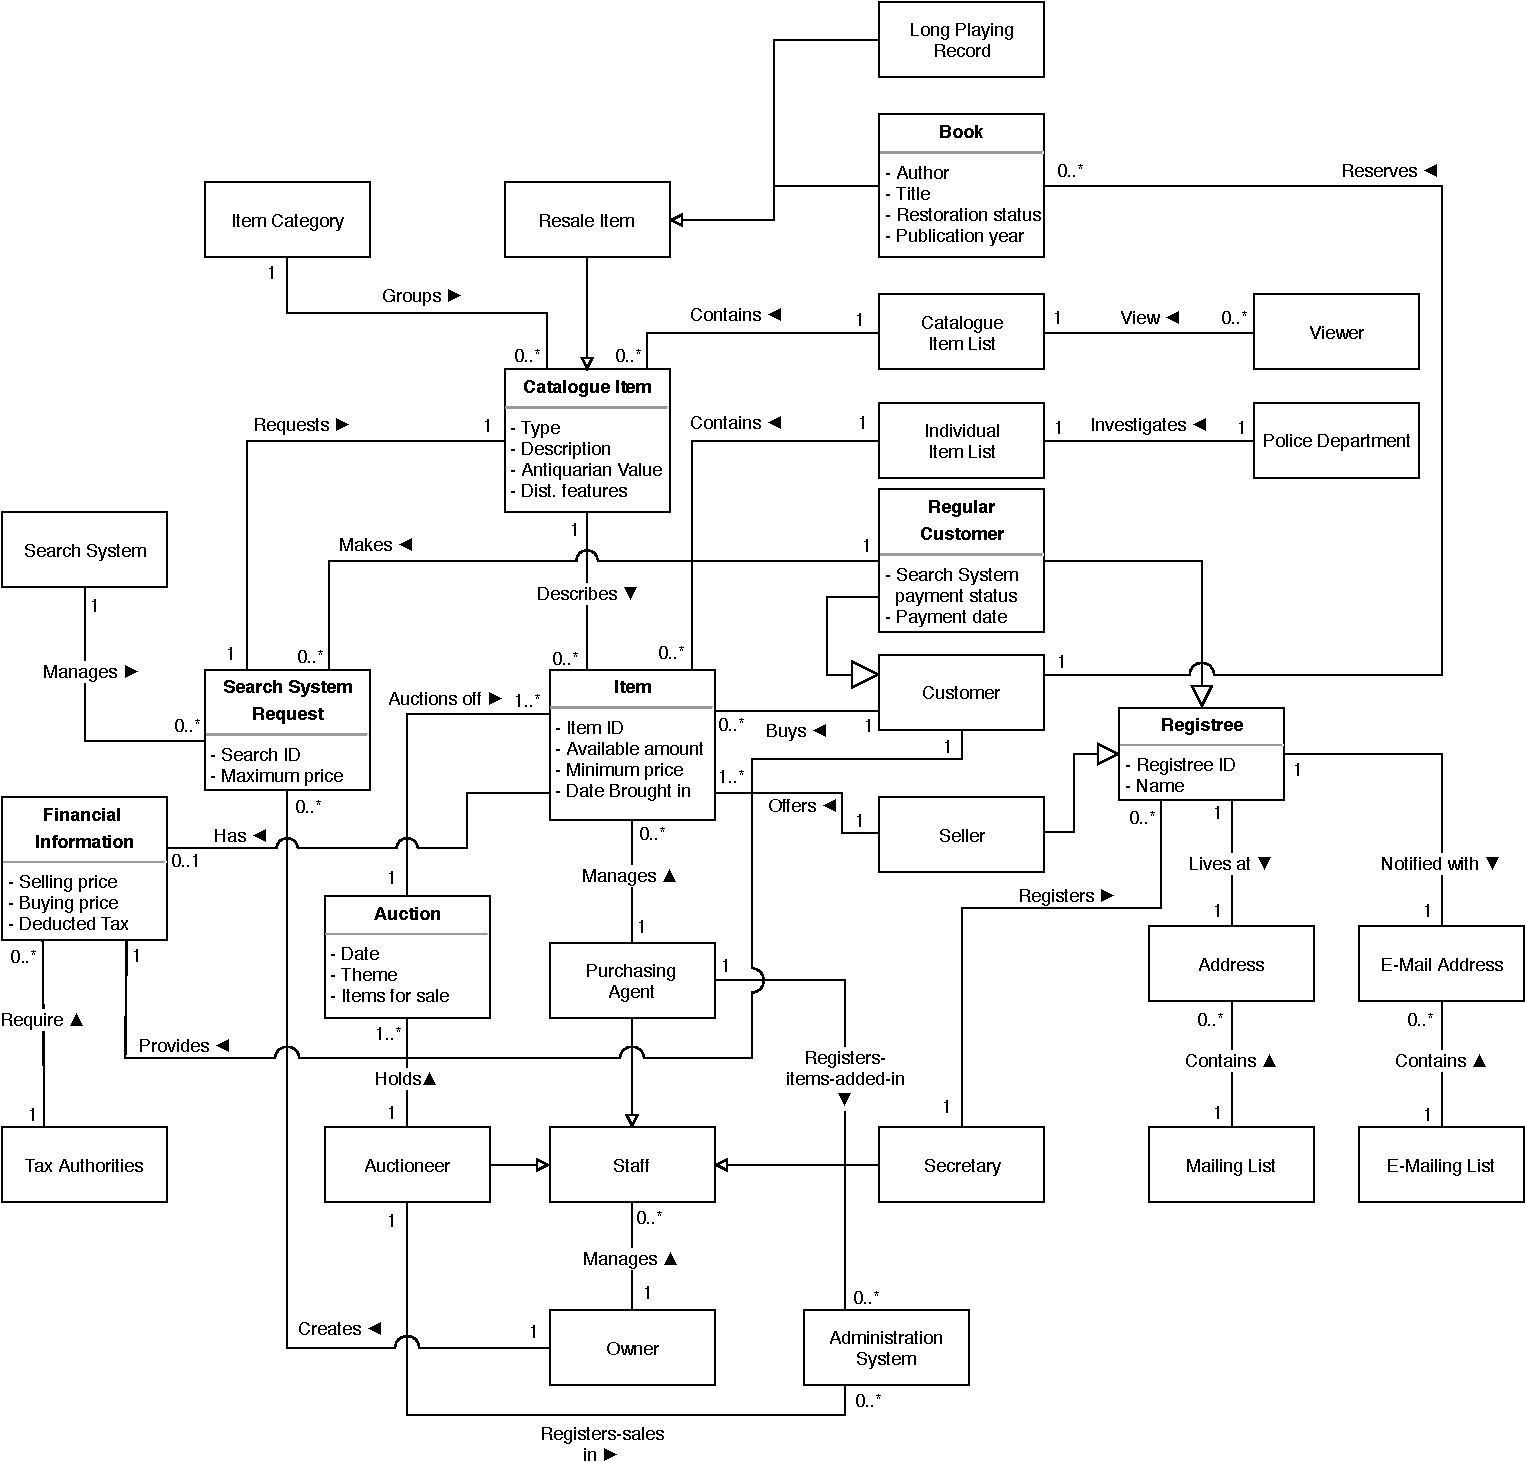
\includegraphics[scale=.9]{uml/domainmodelUPD3.pdf}
\end{figure}
% arrows for domain models to copy: ► ◄ ▲ ▼

% Things to add:
% Search Request, Book (maybe multiple kinds and a catalogue, well see)
The domain model is a universal, graphical representation of the relevant concepts. It shows how all concepts relate to eachother. For example, you can see that items are `used' by a number of sources, such as buyers, sellers, the auctioneer and the purchasing agent. Items are also contained in an item list, which is just the collection of items. The item list can in turn be viewed by the public.\\
We also see that all staff is an instance of the staff class. Any staff is then managed by the owner of The AuctionHouse\textsuperscript{TM}. This does not only make sense for our customer, but also for a future implementation, even though that is not (yet) our concern.\\
We see that a number of parties can register something to the system. One is the secretary can add potential buyers and sellers to the system, granting them more permissions than the general public. Another is the purchasing agent, who can, after evaluation, add items to the system, making them available for viewing by the public.
There is no Auction concept in the domain model. The reason is that auctions are not going to be digitalized; they will still be physically held. Therefore, we do not concern ourselves with it when sketching the domain.
\section{Class Diagram}
\section{References}
\subsection*{Concact with the customer}
\begin{enumerate}[1.]
	\item hello
\end{enumerate}
% \section{About Possible Implementation (optional)}

\end{document}